\section{Appendix}
\label{sec:appendix}

\subsection{Unbiasedness Regressions}
In this Appendix we build on the intuition behind the unbiasedness regressions and the measurement of market inefficiency.
We provide plots from simulated efficienct and inefficient markets, and show how the unbiasedness regressions can be used to measure the degree of inefficiency in the market.

\subsubsection{Simulated Efficient Market}
In this section we simulate an efficient market, where returns are normally distributed with a mean of 0 and a standard deviation of 0.1.
They are independent random events.

\begin{figure}[h]
    \centering
    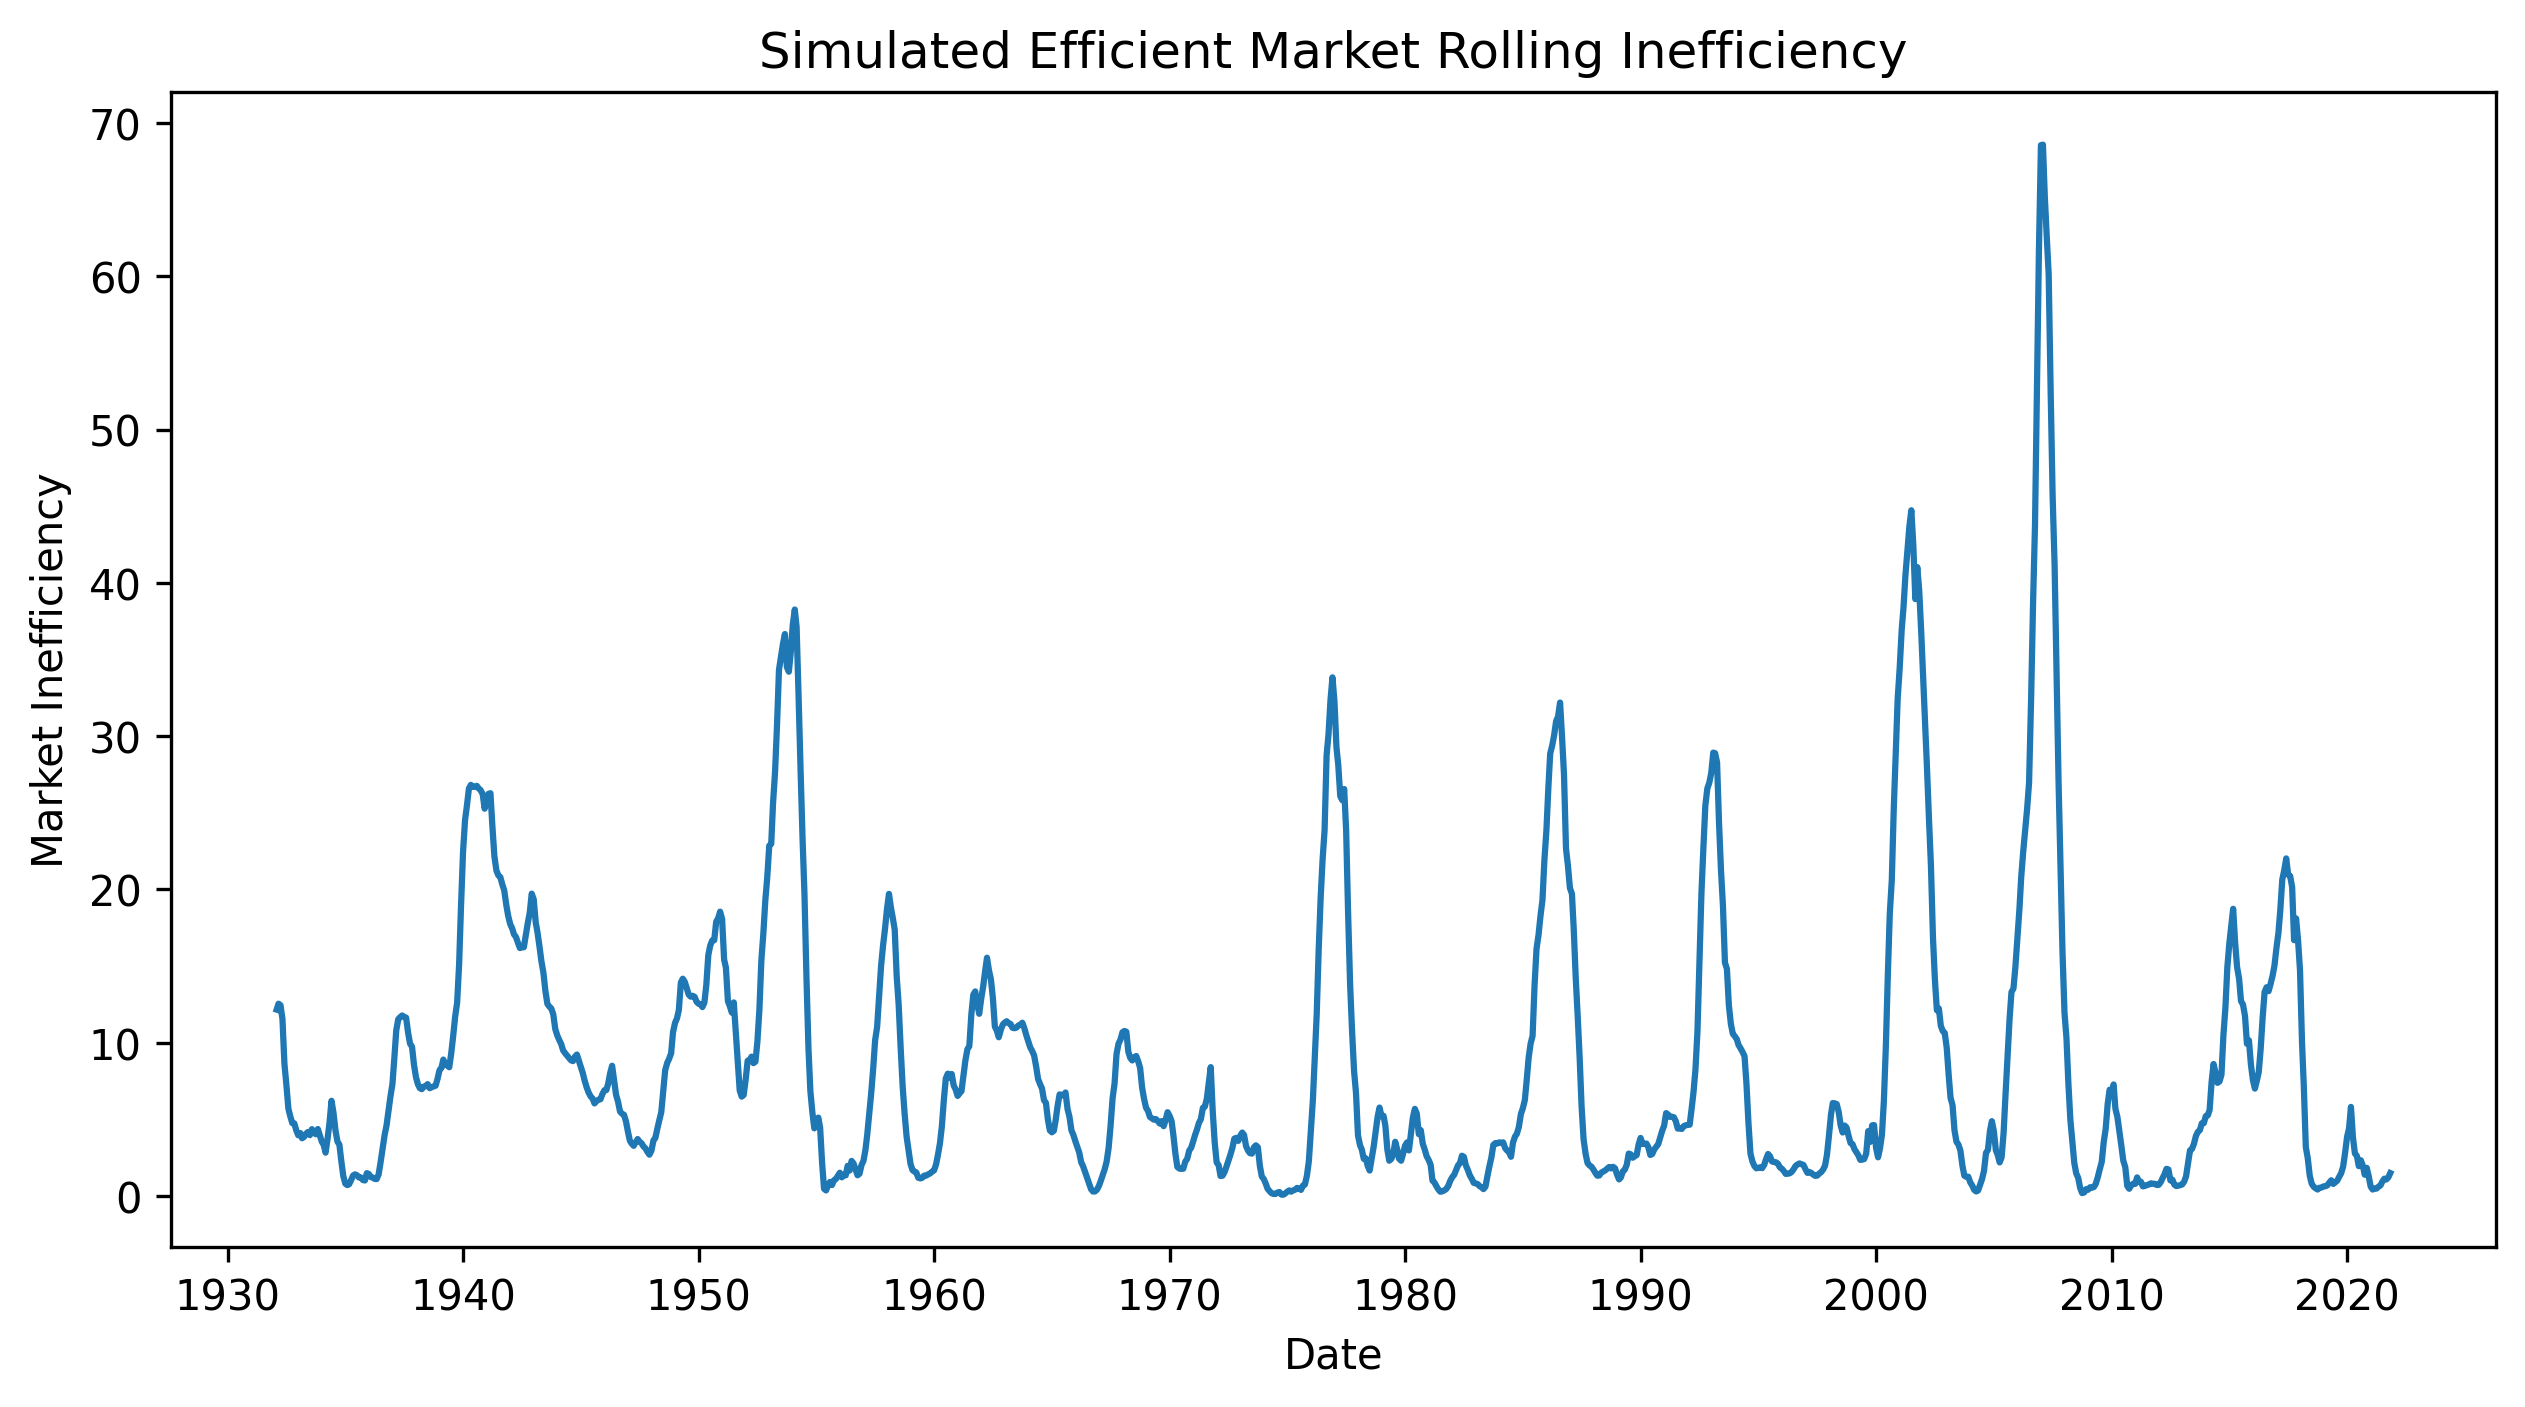
\includegraphics[width=1\textwidth]{../figs/Simulated Efficient Market Rolling Inefficiency.png}
    \caption{Simulated Efficient Market}
    \label{fig:efficient_market}
\end{figure}

In Figure \ref{fig:efficient_market} we see the rolling inefficiency of the simulated efficient market.
Notice that the level remains low, with only small spikes in inefficiency.

\subsubsection{Simulated Inefficient Market}
In this section we simulate an inefficient market, where returns are an AR(1) process:
\begin{equation}
    r_t = \phi r_{t-1} + \epsilon_t
\end{equation}

where $\phi = 0.5$ and $\epsilon_t \sim N(0, 0.1)$. The resuling series of market inefficiency
 is shown in Figure \ref{fig:inefficient_market}. We see that there are much more frequent spikes of inefficiency, and the level of inefficiency is much higher than in the efficient market.

\begin{figure}[h]
    \centering
    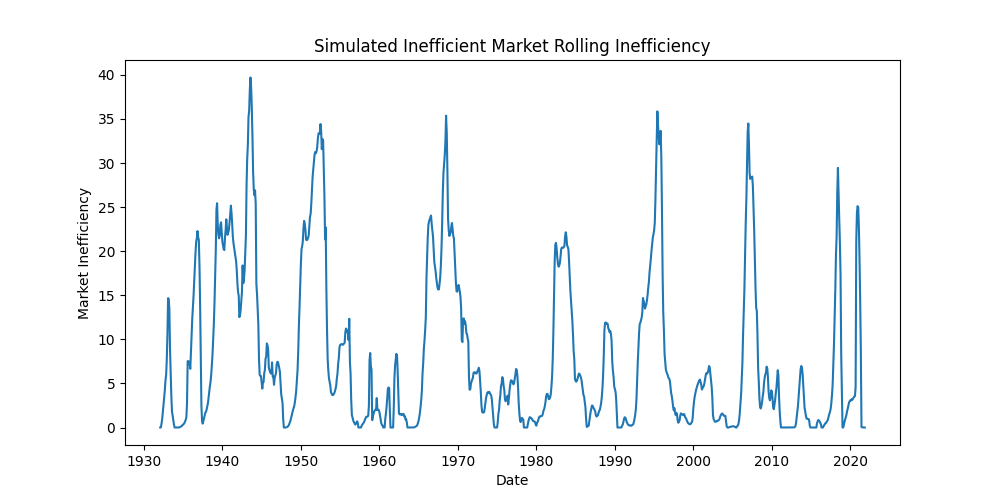
\includegraphics[width=1\textwidth]{../figs/Simulated Inefficient Market Rolling Inefficiency.png}
    \caption{Simulated Inefficient Market}
    \label{fig:inefficient_market}
\end{figure}

\subsubsection{$R^2$ and Intuition Building}
The $R^2$ value of the unbiasedness regression is a measure of how well the partial returns from $0$ to $t$ predict the total return from $t$ to $T$.
While $\beta_t$ measures the efficiency with which the market pricesses information, $R^2$ measures the information content of the partial returns.

I prove an example of the $R^2$ and $\beta_t$ values around 'Earnings Months' and 'Non-Earnings Months' in the SP500. I define
'Earnings Months' as the months where the SP500 companies typically report their earnings (January, April, July, October), and 'Non-Earnings Months' as the remaining months.